% =============================================================================
% CAPÍTULO 5 — volta 1 (AGENTS.md §6): o orçamento é do procedimento, e sobrevive à consulta.
%
% O fracasso que o abre, com número na mão: o par declarado no capítulo do orçamento vale para UMA
% leitura, e o limiar que o assina foi escolhido entre seis olhando o tombo. Rodando a regra de
% escolha dentro de 60 mundos com tombo injetado, o vencedor é o limiar 8 em 45 deles, e o orçamento
% médio do vencedor é de 8,4 anos por alarme contra os 5.084,9 do limiar que o livro imprime.
%
% Medição: lab/experimentos/E31_aposta.ipynb; figuras/E31_aposta_1.pdf; lib/frevolab/aposta.py.
% =============================================================================

\chapter{O orçamento que sobrevive a olhar sempre}\label{cap:aposta}

% aterramento: capital
% aterramento: taxa-de-violacao
% aterramento: razao

O capítulo do orçamento fechou com um par declarado: com que frequência o vigia soa quando nada muda,
e quanto ele demora quando algo muda. O par é de um limiar --- e aquele limiar não caiu do céu: foi
escolhido entre \numApostaLimiares{} olhando os tombos do mercado. Este capítulo faz as duas
perguntas que aquele fecho deixou de pé, e nenhuma das duas é sobre o mundo.

\section{O orçamento é de quem escolhe}

A primeira pergunta é de quem o número é. Nos \numApostaMundosParado{} mundos que nunca mudam, os
seis limiares declaram isto:

\begin{table}[htbp]
  \centering
  \small
  \begin{tabular}{lrrrrrr}
    \hline
    limiar & oito & nove & dez & onze & doze & \numVigiaLimiar \\
    anos por alarme & \numApostaAnosOito & \numApostaAnosNove & \numApostaAnosDez
      & \numApostaAnosOnze & \numApostaAnosDoze & \numApostaAnosTreze \\
    \hline
  \end{tabular}
  \caption{O orçamento de cada um dos \numApostaLimiares{} limiares, medido nos mesmos
    \numApostaMundosParado{} mundos parados. O limiar do livro é o mais raro da família.}
  \label{tab:orcamento-dos-limiares}
\end{table}

O limiar do livro é o mais raro da família por uma razão que não é dele: ele foi escolhido pelo
outro lado da troca. A regra do capítulo anterior é \emph{o limiar que chega mais cedo ao maior
tombo}, e essa regra, rodada dentro de \numApostaMundosTombo{} mundos sorteados com um tombo de
\numApostaTomboDias{} dias injetado num ponto qualquer, escolhe o limiar mais baixo em quase todos
eles --- em \numApostaVencedorOito{} dos \numApostaMundosTombo{}. O orçamento médio do vencedor é de
\numApostaOrcamentoVencedor{} anos por alarme, contra os \numApostaOrcamentoEscolhido{} do limiar
que o livro imprime.

A distância entre esses dois números não é erro de conta: é o preço de escolher olhando o dado. O
limiar \numVigiaLimiar{} é raro porque passou em \emph{duas} provas ao mesmo tempo --- chegar cedo
no tombo que aconteceu, e não soar no mundo que não mudou. Escolher só pela primeira devolve uma
máquina de falso alarme, e é o que a medição mostra: aquele orçamento de milhares de anos é do
\textbf{procedimento}, e não do limiar.

\section{A aposta}

A segunda pergunta é sobre o uso, e ela é pior. Todo aquele orçamento vale para quem pergunta no fim
--- mas ninguém consulta um alarme no fim: consulta-se todo dia, e age-se na primeira vez que ele
soa. Quem olha \numApostaBlocos{} vezes gasta o orçamento \numApostaBlocos{} vezes, e a soma das
chances --- o mesmo teto da união do capítulo do orçamento, agora no tempo --- passa de cem por cento
sem que nada tenha mudado no mundo.

A saída não é olhar menos: é trocar o limiar por um capital. Em cada bloco de \numBlocoDias{} dias
conta-se quantas violações houve, e o bloco vale a razão de verossimilhanças entre o mundo que mudou
e o mundo parado.

\begin{proposicao}[o preço da aposta]\label{prop:aposta}
Seja $V$ o capital acumulado: o produto das razões $R$ de cada bloco, com a taxa de violação $q$ sob
o mundo parado e $q_1$ sob o mundo que mudou. Sob o mundo parado cada razão tem média um, de modo que
o capital é uma martingala, e a desigualdade de Ville dá o orçamento de uma vez para \textbf{todos}
os instantes: a chance de o capital alcançar o inverso da taxa declarada não passa dessa taxa.
\end{proposicao}

\begin{proof}
As violações de blocos que não se sobrepõem são independentes, e a razão do bloco é
$R = (q_1/q)^{L}((1-q_1)/(1-q))^{n-L}$, com $n$ dias no bloco e $L$ violações nele. A média de $R$ é
um --- é a conta que o capítulo do orçamento já fez, bloco a bloco. O produto de variáveis de média
um, com as médias condicionais também um, é uma martingala; e a desigualdade de Ville para
martingalas positivas diz que a chance de o supremo alcançar o inverso da taxa declarada não passa
a afirmação.
\end{proof}

A proposição é a forma exata do que se quer de um alarme: \textbf{um orçamento só, e não um por
olhada}. Ela tem nome na literatura dos testes sequenciais, e é de lá que este livro a traz: o
capital é uma \emph{e-value} acumulada \cite{vovk2021values}, a promessa de valer em qualquer
instante é a inferência \emph{anytime-valid} \cite{wang2025anytime}, a construção a partir de um
modelo preditivo é o \emph{numeraire} \cite{larsson2025numeraire}, e a detecção sequencial que
aprende a mistura enquanto observa é o que se faz hoje com ela \cite{halme2026adaptive}.

\section{O que o capital compra, e o que ele cobra}

\begin{table}[htbp]
  \centering
  \small
  \begin{tabular}{lr}
    \hline
    capital que assina \numApostaAlfa{}\% em qualquer instante & \numApostaCapitalLimiar \\
    mundos parados que cruzam esse capital & \numApostaSoamPct{}\% \\
    capital mediano no fim de um mundo parado & \numApostaCapitalMedianoPct{}\% \\
    atraso para ver uma taxa que dobra & \numApostaLatenciaBlocos{} blocos, \numApostaLatenciaDias{} dias \\
    \hline
  \end{tabular}
  \caption{A aposta medida: o orçamento é respeitado, o capital típico se perde, e a certeza custa
    tempo.}
  \label{tab:aposta}
\end{table}

Três coisas ficam ditas nessa tabela. \textbf{O orçamento é respeitado}: \numApostaSoamPct{}\% dos
mundos parados cruzam o capital, contra os \numApostaAlfa{}\% que Ville promete no máximo. Não é uma
barra frouxa --- é uma barra que vale para sempre, e é isso que o limiar não entrega.

\textbf{O capital típico se perde}, e isso não é defeito: a mediana no fim de um mundo parado é de
\numApostaCapitalMedianoPct{}\% do capital inicial. É o que uma aposta é --- quem aposta contra o
mundo parado perde quase sempre, e quem ganha, ganha muito. A média do capital fica em um, e é a
cauda que paga.

\textbf{E a certeza custa tempo}: uma taxa de violação que dobra leva \numApostaLatenciaBlocos{}
blocos, ou \numApostaLatenciaDias{} dias, para atravessar o capital. O limiar soa no primeiro bloco
que o alcança, e chega antes porque promete menos. É a mesma troca do capítulo do orçamento, medida na
outra ponta: o limiar chega antes e paga em falso alarme, e o capital compra o direito de olhar
sempre pagando em dias.

\begin{figure}[htbp]
  \centering
  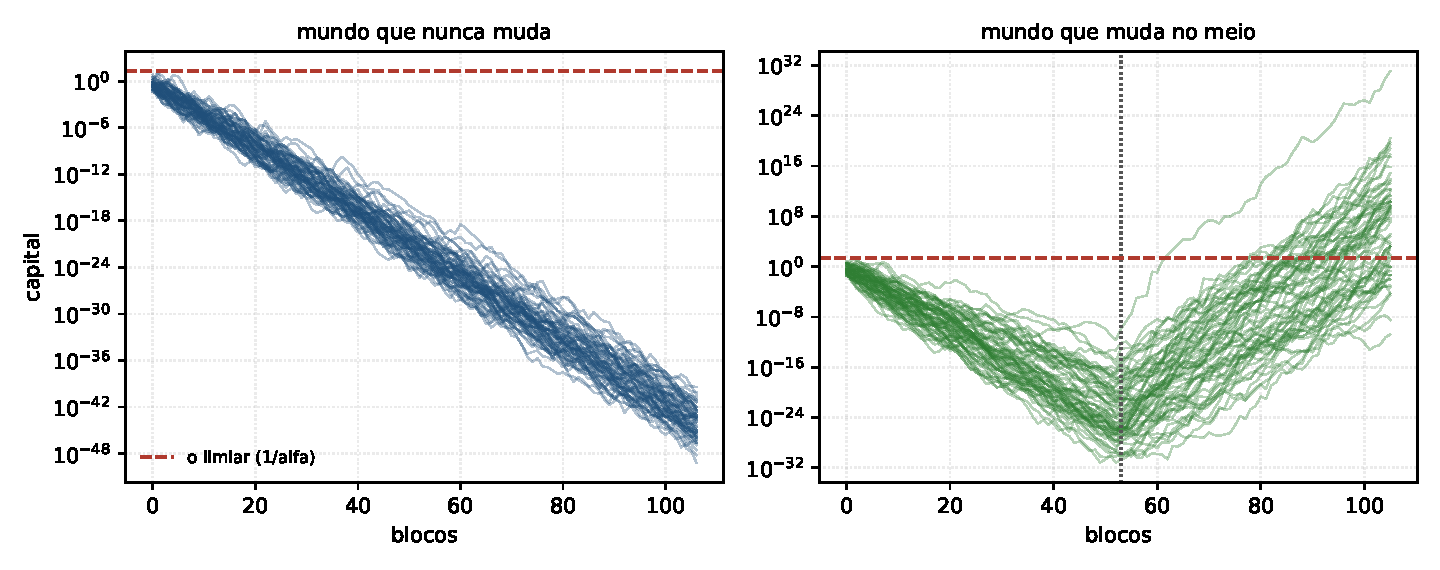
\includegraphics[width=\linewidth]{figuras/E31_aposta_1.pdf}
  \caption{O capital de alguns mundos, no mundo que nunca muda (à esquerda) e no que muda no
    meio (à direita), com o limiar da aposta na linha tracejada. À esquerda as trajetórias caem,
    e só a cauda cruza; à direita elas sobem depois da linha pontilhada, que é o dia da mudança.}
  \label{fig:aposta}
\end{figure}

\section{Quando os blocos falam}

A prova da aposta comprou uma linha barata: «as violações de blocos que não se sobrepõem são
independentes». O mundo não assina essa linha --- os blocos falam entre si, e a mesma pergunta do
início volta pelo cano: o que sobrevive do orçamento quando a estrutura entre as leituras não é a
da prova?

O desenho é o mais honesto possível, porque é o pior possível: \numApostaBlocos{} blocos, cada um
com um p-valor válido na margem --- uniforme, medido: \numFusaoMarginalIndep{} no mundo calado
contra \numFusaoMarginalAcoplado{} no mundo que fala --- e uma amarra declarada entre eles: um
fator comum de gaussianas que correlaciona os blocos sem tocar nenhuma margem. Nada mudou em bloco nenhum; o que mudou é que eles falam. Três fusões competem: o mínimo
de Bonferroni, que não depende de estrutura nenhuma --- a união é a união; a média dos p-valores,
calibrada no mundo calado para entregar exatamente o orçamento; e a média de e-values, cada p-valor
convertido pelo calibrador de média um, com o limiar de Markov em um sobre a taxa --- que também
não depende de estrutura nenhuma.

\begin{figure}[htbp]
  \centering
  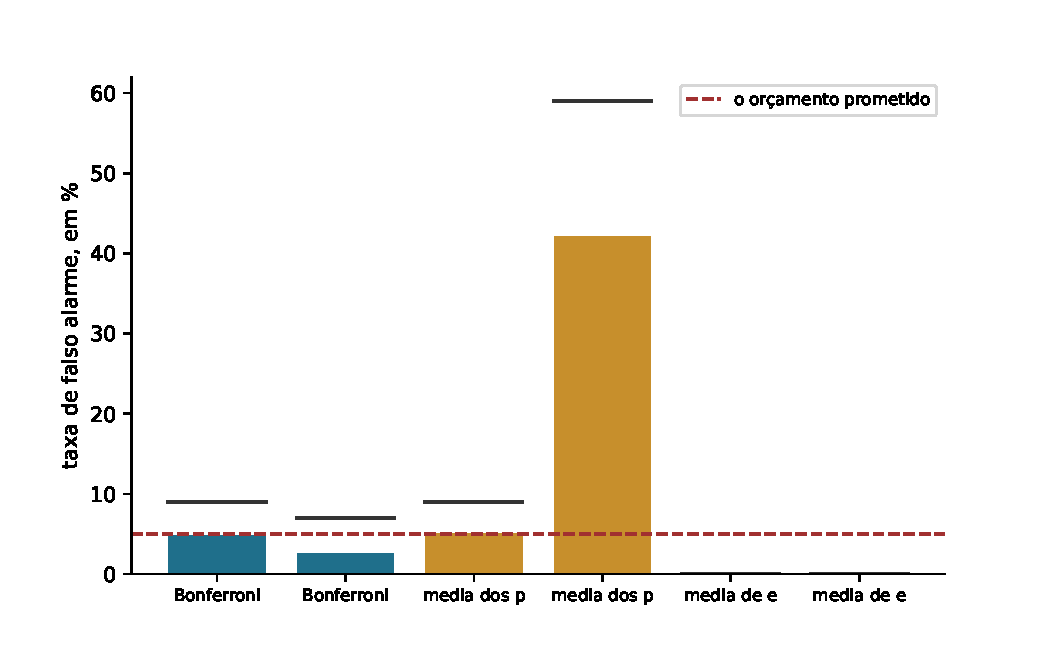
\includegraphics[width=\linewidth]{figuras/E43_fusao_1.pdf}
  \caption{As três fusões nos dois mundos, contra o orçamento prometido (linha tracejada). A média
    dos p-valores entrega o combinado no mundo calado e oito vezes mais no que fala; Bonferroni e a
    média de e-values ficam abaixo da linha nos dois. O traço é o pior lote de sortes.}
  \label{fig:fusao_taxas}
\end{figure}

O número é o da figura: a média dos p-valores entrega \numFusaoMediapIndep{}\% no mundo calado ---
a calibração exata, o orçamento cumprido --- e \numFusaoMediapAcoplado{}\% no mundo que fala, com o
pior lote em \numFusaoMediapAcopladoMax{}\%. O orçamento não dobrou nem triplicou: oito vezes. E as
duas fusões que não pedem estrutura seguram a linha --- Bonferroni com \numFusaoBonferroniIndep{}\%
e \numFusaoBonferroniAcoplado{}\%, a média de e-values com \numFusaoMediaeIndep{}\% e
\numFusaoMediaeAcoplado{}\%, cumprindo com a folga de quem não assumiu nada. Quais fusões de
p-valores são admissíveis quando a amarra entre eles é arbitrária --- e quais não são --- tem
resposta conhecida \cite{vovk2022admissible}, e ela começa por esta: a média dos p não está entre
elas. Do lado das apostas, o capital que segue válido estimando quando os blocos falam é a mesma família
de e-values que este capítulo chama de capital \cite{waudbysmith2024estimating}.

\begin{figure}[htbp]
  \centering
  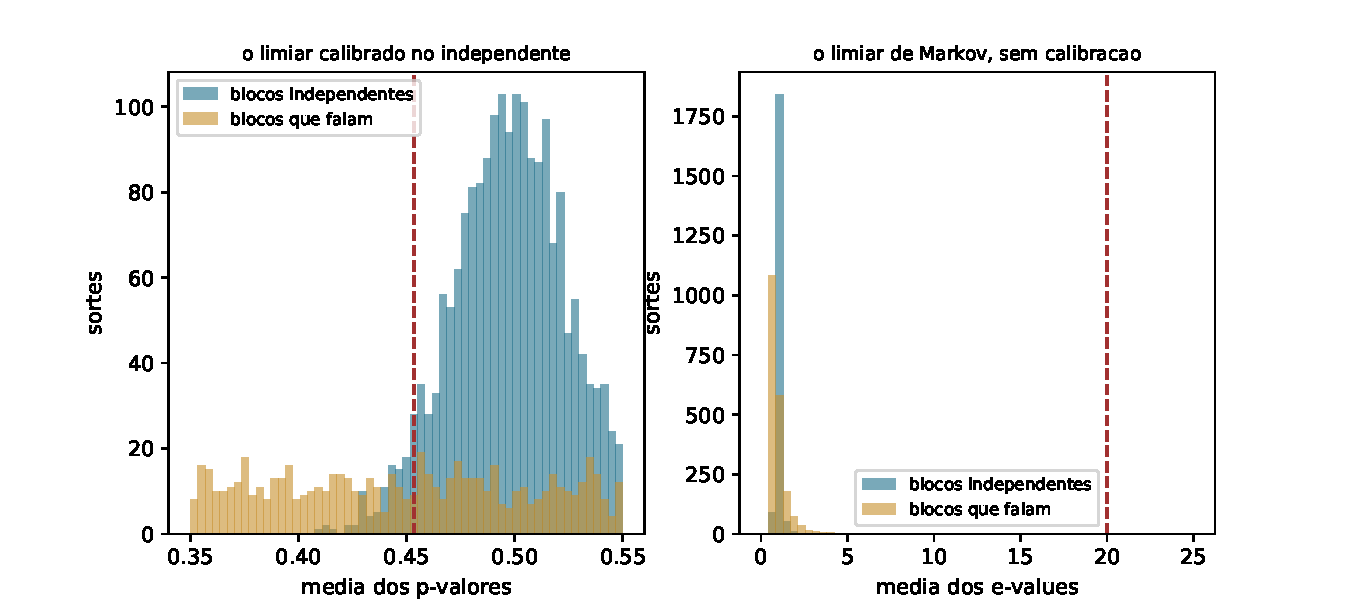
\includegraphics[width=\linewidth]{figuras/E43_fusao_2.pdf}
  \caption{Por que uma rompe e as outras não. À esquerda, a média dos p-valores nos dois mundos:
    o mundo que fala é mais largo, e a massa à esquerda do limiar calibrado --- o falso alarme ---
    cresce de graça. À direita, a média dos e-values nos mesmos mundos: as duas distribuições
    ficam longe do limiar vermelho.}
  \label{fig:fusao_distribuicoes}
\end{figure}

O capítulo fechou com um orçamento que sobrevive a ser lido todo dia; esta seção fecha com o que
sobrevive a mais: os blocos falarem entre si. Sobrevive --- desde que a fusão não case os
p-valores como se o mundo fosse calado, e é a moeda do capítulo, a e-value, a que não precisa de
silêncio para valer um.
\section{O que fica}

Fica a correção do instrumento, e ela vale para todo alarme do livro: \textbf{o orçamento declarado é
o do procedimento que escolhe, e não o do limiar escolhido} --- e ele tem de sobreviver à consulta,
que é diária. Um alarme que se lê todo dia ou declara o capital que gasta, ou está prometendo um
número que não é dele.

E fica o fracasso seguinte, que a curva da troca não mostra e este capítulo também não: as duas
medições foram feitas com o tombo, e o tombo é a forma de mudança mais fácil de ver. O mundo muda de
outras maneiras.
